\documentclass[twoside]{article}% \usepackage{aistats2017}

% FONTS
\usepackage[T1]{fontenc}
\usepackage{tgtermes}
\usepackage{amsmath}
\usepackage{enumitem}

% Font choice 1:
\usepackage[subscriptcorrection,
           amssymbols,
           mtpbb,
           mtpcal,
           nofontinfo  % suppresses all warnings
          ]{mtpro2}

% Font choice 2:
%\usepackage[scaled=0.92]{PTSans}
%\usepackage{amssymb}
%\newcommand{\mathbold}[1]{\ensuremath{\boldsymbol{\mathbf{#1}}}}
%\newcommand{\mbf}[1]{\ensuremath{\boldsymbol{\mathbf{#1}}}}
%\newcommand{\hmbtheta}{\mathbold{\widehat{\theta}}}
%\newcommand{\hb}{\mathbold{\widehat{b}}}
%\newcommand{\hB}{\mathbold{\widehat{B}}}
%\newcommand{\hbP}{\mathbold{\widehat{P}}}

\usepackage{scalefnt,letltxmacro}
\LetLtxMacro{\oldtextsc}{\textsc}
\renewcommand{\textsc}[1]{\oldtextsc{\scalefont{1.10}#1}}

% \renewcommand*\ttdefault{lmvtt}
\usepackage[ttdefault=true]{AnonymousPro}

% GEOMETRY
%\usepackage[
%  paper  = letterpaper,
%  left   = 1.65in,
%  right  = 1.65in,
%  top    = 1.0in,
%  bottom = 1.0in,
%  ]{geometry}

% COLOR
\usepackage[usenames,dvipsnames]{xcolor}
\definecolor{shadecolor}{gray}{0.9}

% SPACING and TEXT
%\usepackage[final,expansion=alltext]{microtype}
\usepackage[english]{babel}
\usepackage[parfill]{parskip}
\usepackage{afterpage}
\usepackage{framed}

%redefine the leftbar environment to accept a width and coloring options
\renewenvironment{leftbar}[1][\hsize]
{%
  \def\FrameCommand
  {%
    {\color{Gray}\vrule width 3pt}%
    \hspace{10pt}%
    %\hspace{0pt}\fboxsep=\FrameSep\colorbox{black!10}%
  }%
  \MakeFramed{\hsize#1\advance\hsize-\width\FrameRestore}%
}%
{\endMakeFramed}

% define a paragraph header function
\DeclareRobustCommand{\parhead}[1]{\textbf{#1}~}

% EDITING
% line numbering in left margin
\usepackage{lineno}
\renewcommand\linenumberfont{\normalfont

             \footnotesize
                             \sffamily
                             \color{SkyBlue}}
% ragged paragraphs in right margin
\usepackage{ragged2e}
\DeclareRobustCommand{\sidenote}[1]{\marginpar{
                                    \RaggedRight
                                    \textcolor{Plum}{\textsf{#1}}}}
% paragraph counter in right margin
\newcommand{\parnum}{\bfseries\P\arabic{parcount}}
\newcounter{parcount}
\newcommand\p{%
    \stepcounter{parcount}%
    \leavevmode\marginpar[\hfill\parnum]{\parnum}%
}
% paragraph helper
\DeclareRobustCommand{\PP}{\textcolor{Plum}{\P} }

% COUNTERS
\renewcommand{\labelenumi}{\color{black!67}{\arabic{enumi}.}}
\renewcommand{\labelenumii}{{\color{black!67}(\alph{enumii})}}
\renewcommand{\labelitemi}{{\color{black!67}\textbullet}}

% FIGURES
\usepackage{graphicx}
\usepackage[labelfont=bf]{caption}
\usepackage[format=hang]{subcaption}

% TABLES
\usepackage{booktabs}

% ALGORITHMS
\usepackage[algoruled]{algorithm2e}
\usepackage{listings}
\usepackage{fancyvrb}
\fvset{fontsize=\normalsize}

% BIBLIOGRAPHY
\usepackage[numbers]{natbib}

% HYPERREF
\usepackage[colorlinks,linktoc=all]{hyperref}
%\usepackage[all]{hypcap}
\hypersetup{citecolor=Blue}
\hypersetup{linkcolor=MidnightBlue}
\hypersetup{urlcolor=MidnightBlue}

% ##### CLEVERREF
\usepackage[nameinlink]{cleveref}
\creflabelformat{equation}{#1#2#3}

% CLEVEREF alternative
\newcommand{\myeqp}[1]{Eq.\ref{eq:#1}}
\newcommand{\mysec}[1]{Section~\ref{sec:#1}}
\newcommand{\mytable}[1]{Table~\ref{table:#1}}
\newcommand{\myfig}[1]{Figure~\ref{fig:#1}}
\newcommand{\myappendix}[1]{Appendix \ref{appendix:#1}}
\newcommand{\myalg}[1]{Algorithm~\ref{alg:#1}}

% ACRONYMS
\usepackage
[acronym,smallcaps,nowarn,section,nogroupskip,nonumberlist]{glossaries}
\glsdisablehyper{}
% \makeglossaries

% COLOR DEFINITIONS
\newcommand{\red}[1]{\textcolor{BrickRed}{#1}}
\newcommand{\orange}[1]{o\textcolor{BurntOrange}{#1}}
\newcommand{\green}[1]{\textcolor{OliveGreen}{#1}}
\newcommand{\blue}[1]{\textcolor{MidnightBlue}{#1}}
\newcommand{\gray}[1]{\textcolor{black!60}{#1}}

% LISTINGS DEFINTIONS
\lstdefinestyle{mystyle}{
    commentstyle=\color{OliveGreen},
    keywordstyle=\color{BurntOrange},
    numberstyle=\tiny\color{black!60},
    stringstyle=\color{MidnightBlue},
    basicstyle=\ttfamily,
    breakatwhitespace=false,
    breaklines=true,
    captionpos=b,
    keepspaces=true,
    numbers=left,
    numbersep=5pt,
    showspaces=false,
    showstringspaces=false,
    showtabs=false,
    tabsize=2
}
\lstset{style=mystyle}

%\usepackage{titlesec}
%\titlespacing*{\section}{0pt}{1.1\baselineskop}{\baselineskip}

% A
\newacronym{ADVI}{advi}{automatic differentiation variational inference}

% B
\newacronym{BBVI}{bbvi}{black-box variational inference}

% C
\newacronym{CTM}{ctm}{correlated topic model}

% D
\newacronym[\glslongpluralkey={deep exponential families}]{DEF}{def}{deep exponential family}
\newacronym{DMIS}{dmis}{deterministic multiple importance sampling}

% E
\newacronym{ELBO}{elbo}{evidence lower bound}

% G
\newacronym{GNTS}{gn-ts}{gamma-normal time series model}
\newacronym{G-REP}{g-rep}{generalized reparameterization}

% K
\newacronym{KL}{kl}{{K}ullback-{L}eibler}

% L
\newacronym{LDA}{lda}{latent {D}irichlet allocation}

% M
\newacronym{MF}{mf}{matrix factorization}
\newacronym{MIS}{mis}{multiple importance sampling}
\newacronym{MATLAB}{matlab}{MATLAB}

\newacronym{NIPS}{nips}{Neural Information Processing Systems}

% O
\newacronym{OBBVI}{o-bbvi}{overdispersed black-box variational inference}

% R
\newacronym{RS-VI}{rsvi}{rejection sampling variational inference}

% S
\newacronym{SVI}{svi}{stochastic variational inference}

% V
\newacronym{VI}{vi}{variational inference}


% If your paper is accepted, change the options for the package
% aistats2017 as follows:
%
\usepackage[accepted]{aistats2017}
%
% This option will print headings for the title of your paper and
% headings for the authors names, plus a copyright note at the end of
% the first column of the first page.


\begin{document}

% If your paper is accepted and the title of your paper is very long,
% the style will print as headings an error message. Use the following
% command to supply a shorter title of your paper so that it can be
% used as headings.
%
%\runningtitle{I use this title instead because the last one was very long}

% If your paper is accepted and the number of authors is large, the
% style will print as headings an error message. Use the following
% command to supply a shorter version of the authors names so that
% they can be used as headings (for example, use only the surnames)
%
%\runningauthor{Surname 1, Surname 2, Surname 3, ...., Surname n}

\twocolumn[

\aistatstitle{Supplementary Material}

\aistatsauthor{Christian A. Naesseth$^{\dagger\ddagger}$ \And Francisco J. R. Ruiz$^{\ddagger\S}$ \And Scott W. Linderman$^{\ddagger}$  \And David M. Blei$^{\ddagger}$}

\aistatsaddress{$^\dagger$Link\"oping University~~$^\ddagger$Columbia University~~$^\S$University of Cambridge} ]

% ======================================================================
%                           Introduction
% ======================================================================
%\section{Supplementary Material}
\section{Distribution of $\eps$}
Here we formalize the claim in the main manuscript regarding the distribution of the accepted variable $\eps$ in the rejection sampler. Recall that ${z=h(\eps,\theta), ~\eps \sim s(\eps)}$ is equivalent to $z\sim r(z\g\theta)$, and that $q(z\g\theta) \leq M_\theta r(z\g\theta)$. For simplicity we consider the univariate continuous case in the exposition below, but the result also holds for the discrete and multivariate settings. The cumulative distribution function for the accepted $\eps$ is given by
\begin{align*}
\begin{split}
&\Prb(E \leq \eps) = \sum_{i=1}^\infty \Prb(E \leq \eps, E = E_i)\\
&= \sum_{i=1}^\infty \Bigg[ \Prb\left(E_i \leq \eps, U_i < \frac{q(h(E_i,\theta)\g\theta)}{M_\theta r(h(E_i,\theta)\g\theta)}\right)\\
&\quad\prod_{j=1}^{i-1} \Prb\left(U_j \geq \frac{q(h(E_j,\theta)\g\theta)}{M_\theta r(h(E_j,\theta)\g\theta)}\right)\Bigg] \\
&= \sum_{i=1}^\infty \int_{-\infty}^\eps s(e) \frac{q(h(e,\theta)\g\theta)}{M_\theta r(h(e,\theta)\g\theta)} \myd e \prod_{j=1}^{i-1} \left(1-\frac{1}{M_\theta}\right)\\
&= \int_{-\infty}^\eps s(e) \frac{q(h(e,\theta)\g\theta)}{r(h(e,\theta)\g\theta)} \myd e \cdot \frac{1}{M_\theta} \cdot \sum_{i=1}^\infty  \left(1-\frac{1}{M_\theta}\right)^{i-1}\\
&= \int_{-\infty}^\eps s(e) \frac{q(h(e,\theta)\g\theta)}{r(h(e,\theta)\g\theta)}\myd e.
\end{split}
\end{align*}
Here, we have applied that ${z=h(\eps,\theta), ~\eps \sim s(\eps)}$ is a reparameterization of $z\sim r(z\g\theta)$, and thus
\begin{align*}
\begin{split}
& \Prb\left(U_j \geq \frac{q(h(E_j,\theta)\g\theta)}{M_\theta r(h(E_j,\theta)\g\theta)}\right) \\
& = \int_{-\infty}^{\infty} s(e)\left( 1- \frac{q(h(e,\theta)\g\theta)}{M_\theta r(h(e,\theta)\g\theta)}\right) \myd e \\
& = 1-\frac{1}{M_\theta}\E_{s(e)}\left[ \frac{q(h(e,\theta)\g\theta)}{r(h(e,\theta)\g\theta)}\right] \\
& = 1-\frac{1}{M_\theta}\E_{r(z\g \theta)} \left[ \frac{q(z\g\theta)}{r(z\g\theta)} \right] = 1-\frac{1}{M_\theta}.
\end{split}
\end{align*}

The density is obtained by taking the derivative of the cumulative distribution function with respect to $\eps$,
\begin{align*}
\frac{\myd }{\myd \eps} \Prb(E \leq \eps) =  s(\eps) \frac{q(h(\eps,\theta)\g\theta)}{r(h(\eps,\theta)\g\theta)},
\end{align*}
which is the expression from the main manuscript.

The motivation from the main manuscript is basically a standard ``area-under-the-curve'' or geometric argument for rejection sampling \citep{robert2004monte}, but for $\eps$ instead of $z$.


\section{Derivation of the Gradient}\label{sec:gradient}
We provide below details for the derivation of the gradient. We assume that $h$ is differentiable (almost everywhere) with respect to $\theta$, and that ${f(h(\eps,\theta))\frac{q(h(\eps,\theta)\g\theta)}{r(h(\eps,\theta)\g\theta)}}$ is continuous in $\theta$ for all $\eps$. Then, we have
\begin{align*}
\begin{split}
&\grad_\theta \E_{q(z\g \theta)}[f(z)] = \grad_\theta \E_{\pi(\eps\g\theta)}[f(h(\eps,\theta))] \\
&= \int s(\eps) \grad_\theta \left( f\left(h(\eps,\theta)\right)  \frac{q\left(h(\eps,\theta)\g \theta\right)}{r\left(h(\eps,\theta)\g \theta\right)}  \right) \myd \eps\\
&= \int s(\eps)  \frac{q\left(h(\eps,\theta)\g \theta\right)}{r\left(h(\eps,\theta)\g \theta\right)}  \grad_\theta f\left(h(\eps,\theta)\right)  \myd \eps\\
&+ \int s(\eps) f\left(h(\eps,\theta)\right)  \grad_\theta \left( \frac{q\left(h(\eps,\theta)\g \theta\right)}{r\left(h(\eps,\theta)\g \theta\right)} \right) \myd \eps\\
&= \underbrace{\E_{\pi(\eps\g\theta)}[\grad_\theta f(h(\eps,\theta))]}_{\defeq g_{\text{rep}}}+ \\
&\quad + \underbrace{\E_{\pi(\eps\g\theta)}\left[ f(h(\eps,\theta)) \grad_\theta  \log \frac{q(h(\eps,\theta)\g \theta)}{r(h(\eps,\theta)\g \theta)} \right]}_{\defeq g_{\text{cor}}},
\end{split}
\end{align*}
where in the last step we have identified $\pi(\eps\g\theta)$ and made use of the log-derivative trick
\begin{align*}
 \grad_\theta \frac{q\left(h(\eps,\theta)\g \theta\right)}{r\left(h(\eps,\theta)\g \theta\right)} = \frac{q\left(h(\eps,\theta)\g \theta\right)}{r\left(h(\eps,\theta)\g \theta\right)} \grad_\theta \log \frac{q\left(h(\eps,\theta)\g \theta\right)}{r\left(h(\eps,\theta)\g \theta\right)}.
\end{align*}

\paragraph{Gradient of Log-Ratio in $g_{\text{cor}}$}
For invertible reparameterizations we can simplify the evaluation of the gradient of the log-ratio in $g_{\text{cor}}$ as follows using standard results on transformation of a random variable
\begin{align*}
&\grad_\theta  \log \frac{q(h(\eps,\theta)\g \theta)}{r(h(\eps,\theta)\g \theta)}  = \grad_\theta  \log q(h(\eps,\theta)\g \theta) +\nonumber\\
& +\grad_\theta \log \left| \frac{d h}{d\eps}(\eps,\theta) \right|- \grad_\theta \log \underbrace{s(h^{-1}(h(\eps,\theta),\theta))}_{= ~s(\eps)}\\
&=\grad_\theta  \log q(h(\eps,\theta)\g \theta) + \grad_\theta \log \left| \frac{d h}{d\eps}(\eps,\theta) \right|.
\end{align*}
%\begin{figure*}[t]
  %\centering
  %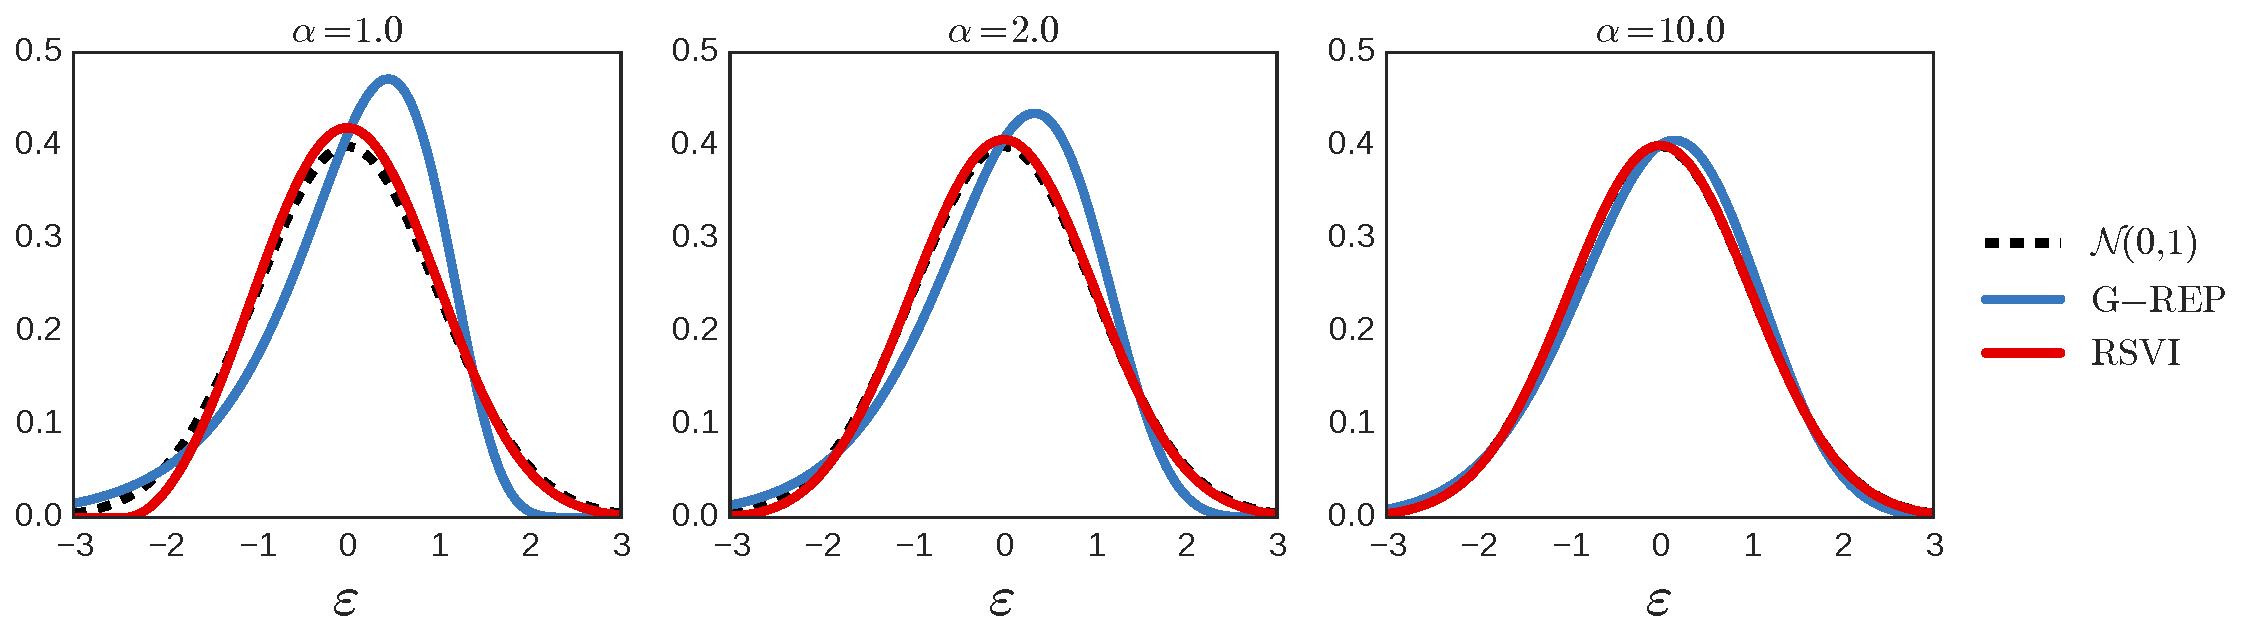
\includegraphics[width=2.\columnwidth]{compare_Qeps} 
  %\caption{Corresponding distribution on $\eps$ for $\alpha = \{1,2,10\}$. We show the transformation suggested by \citet{RuizTB2016}, \gls{G-REP}, and ours inspired by the rejection sampler.}
  %\label{fig:compare_qeps}
%\end{figure*}

%\begin{landscape}


\renewcommand{\arraystretch}{2.5}
\begin{table*}[t]
\centering
\begin{tabular}{ccc} 
\toprule
$q(z\g\theta)$ & $h(\eps,\theta)$ & $s(\eps)$\\
\hline
% GAMMA
$\gam(\alpha,1)$ &$\left(\alpha-\frac{1}{3}\right) \left(1+\frac{\eps}{\sqrt{9\alpha-3}}\right)^3$ & $\eps\sim\N(0,1)$\\
% Truncated Noraml
$\tN(0,1,a,\infty)$ & $\sqrt{a^2-2\log \eps}$ & $\eps \sim \uni[0,1]$\\
% VON MISES
$\mises(\kappa)$ & $\frac{\sign(\eps)}{\cos\left( \frac{1+c\cos(\pi \eps)}{c+\cos(\pi\eps)} \right)}$, $c = \frac{1+\rho^2}{2\rho}$, $\rho = \frac{r-\sqrt{2r}}{2\kappa}$, $r = 1+\sqrt{1+4\kappa^2}$ & $\eps \sim \uni[-1,1]$ \\ \bottomrule
\end{tabular}
\caption{Examples of reparameterizable rejection samplers; many more can be found in \citet{devroye1986}. The first column is the distribution, the second column is the transformation $h(\eps,\theta)$, and the last column is the proposal $s(\eps)$.\label{tab:rep_rejsamplers}}
\end{table*}

\begin{table*}[t]
\centering
\begin{tabular}{ccc}
\toprule
$q(z\g\theta)$ & $g(\tilde z, \theta)$ &  $p(\tilde z\g\theta)$\\
\hline
% BETA
$\bet(\alpha,\beta)$ & $\displaystyle\frac{\tilde z_1}{\tilde z_1 + \tilde z_2}$ & $\tilde z_1 \sim \gam(\alpha,1)$, $\tilde z_2  \sim \gam(\beta,1)$\\%$\frac{\left(\alpha-\frac{1}{3}\right) \left(1+\frac{\eps_1}{\sqrt{9\alpha-3}}\right)^3}{\left(\alpha-\frac{1}{3}\right) \left(1+\frac{\eps_1}{\sqrt{9\alpha-3}}\right)^3+\left(\beta-\frac{1}{3}\right) \left(1+\frac{\eps_2}{\sqrt{9\beta-3}}\right)^3}$\\
% DIRICHLET
$\diri(\alpha_{1:K})$ &$\displaystyle\frac{1}{\sum_\ell \tilde z_\ell} \left(\tilde z_1,\ldots,\tilde z_K\right)^\top$ & $\tilde z_k \sim \gam(\alpha_k,1), ~k=1,\ldots,K$\\
% STUDENT'S T 
$\St(\nu)$ & $\displaystyle\sqrt{\frac{\nu}{2 \tilde z_1}} \tilde z_2$ & $\tilde z_1 \sim \gam(\nu/2,1)$, $\tilde z_2 \sim \N(0,1)$\\
% CHI SQUARED
$\chi^2(k)$ & $\displaystyle2\tilde z$& $\tilde z \sim \gam(k/2,1)$\\
% F
$\fdist(d_1,d_2)$ & $\displaystyle\frac{d_2 \tilde z_1}{d_1 \tilde z_2}$ & $\tilde z_1 \sim \gam(d_1/2,1)$, $\tilde z_2  \sim \gam(d_2/2,1)$\\
% NAKAGAMI
$\nakagami(m,\Omega)$ & $\displaystyle \sqrt{\frac{\Omega\tilde z}{m}}$ & $\tilde z \sim \gam(m,1)$ \\ \bottomrule
\end{tabular}
\caption{Examples of random variables as functions of auxiliary random variables with reparameterizable distributions. The first column is the distribution, the second column is a function $g(\tilde{z},\theta)$ mapping from the auxiliary variables to the desired variable, and the last column is the distribution of the auxiliary variables $\tilde z$.\label{tab:aux_rejSamplers}}
\end{table*}
%\end{landscape}

\section{Examples of Reparameterizable Rejection Samplers}

We show in Table~\ref{tab:rep_rejsamplers} some examples of reparameterizable rejection samplers for three distributions, namely, the gamma, the truncated normal, and the von Misses distributions (for more examples, see \citet{devroye1986}). We show the distribution $q(z\g \theta)$, the transformation $h(\eps,\theta)$, and the proposal $s(\eps)$ used in the rejection sampler.

We show in Table~\ref{tab:aux_rejSamplers} six examples of distributions that can be reparameterized in terms of auxiliary gamma-distributed random variables. We show the distribution $q(z\g\theta)$, the distribution of the auxiliary gamma random variables $p(\tilde{z}\g\theta)$, and the mapping $z=g(\tilde{z},\theta)$.


%\begin{landscape}
%\renewcommand{\arraystretch}{2.5}
%\begin{table}[h]
%\centering
%\caption{Examples of reperameterizable rejection samplers. First column distribution with parameter, second column is function $h$, third column is internal rejection proposal for $\eps$, last column denotes the rejection sampler to be used when generating $\eps$, respectively.}
%\begin{tabular}{c | c | c | c}
%$q(z|\theta)$ & $h(\eps,\theta)$ & $s(\eps)$ & Rejection Sampler\\
%\hline
%% GAMMA
%$\gam(\alpha,1)$ &$\left(\alpha-\frac{1}{3}\right) \left(1+\frac{\eps}{\sqrt{9\alpha-3}}\right)^3$ & $\eps\sim\N(0,1)$ & $\gam(\alpha,1)$\\
%% BETA
%$\bet(\alpha,\beta)$ &$\frac{\left(\alpha-\frac{1}{3}\right) \left(1+\frac{\eps_1}{\sqrt{9\alpha-3}}\right)^3}{\left(\alpha-\frac{1}{3}\right) \left(1+\frac{\eps_1}{\sqrt{9\alpha-3}}\right)^3+\left(\beta-\frac{1}{3}\right) \left(1+\frac{\eps_2}{\sqrt{9\beta-3}}\right)^3}$ & $\eps_1\sim\N(0,1),~\eps_2\sim\N(0,1)$ & $\gam(\alpha,1), \gam(\beta,1)$\\
%% DIRICHLET
%$\diri(\alpha_{1:K})$ &$ \frac{\left(\left(\alpha_1-\frac{1}{3}\right) \left(1+\frac{\eps_1}{\sqrt{9\alpha_1-3}}\right)^3,\ldots,\left(\alpha_K-\frac{1}{3}\right) \left(1+\frac{\eps_K}{\sqrt{9\alpha_K-3}}\right)^3\right)^\top}{\sum_\ell \left(\alpha_\ell-\frac{1}{3}\right) \left(1+\frac{\eps_\ell}{\sqrt{9\alpha_\ell-3}}\right)^3}  $ & $\eps_k\iidsim\N(0,1),~k=1,\ldots,K$ & $\gam(\alpha_k,1)$\\
%% STUDENT'S T 
%$\St(\nu)$ & $e \sqrt{\nu} \left(2\left(\frac{\nu}{2}-\frac{1}{3}\right) \left(1+\frac{\eps}{\sqrt{9\frac{\nu}{2}-3}}\right)^3\right)^{-1/2} $, $e\sim \N(0,1)$ & $\eps\sim\N(0,1)$ & $\gam(\nu/2,1)$\\
%% F
%$\fdist(d_1,d_2)$ & $\frac{d_2 \left(\frac{d_1}{2}-\frac{1}{3}\right) \left(1+\frac{\eps_1}{\sqrt{9\frac{d_1}{2}-3}}\right)^3}{d_1 \left(\frac{d_2}{2}-\frac{1}{3}\right) \left(1+\frac{\eps_2}{\sqrt{9\frac{d_2}{2}-3}}\right)^3}$ & $\eps_1\sim\N(0,1),~\eps_2\sim\N(0,1)$ & $\gam(\frac{d_1}{2},1), \gam(\frac{d_2}{2},1)$\\
%% VON MISES
%$\mises(\kappa)$ & $\frac{\sign(\eps)}{\cos\left( \frac{1+c\cos(\pi \eps)}{c+\cos(\pi\eps)} \right)}$, $c = \frac{1+\rho^2}{2\rho}$, $\rho = \frac{r-\sqrt{2r}}{2\kappa}$, $r = 1+\sqrt{1+4\kappa^2}$ & $\eps \sim \uni[-1,1]$ & $\mises(\kappa)$
%\end{tabular}
%\end{table}
%\end{landscape}

\section{Reparameterizing the Gamma Distribution}
We provide details on reparameterization of the gamma distribution. In the following we consider rate $\beta=1$. Note that this is not a restriction, we can always reparameterize the rate. The density of the gamma random variable is given by
\begin{align*}
q(z\g\alpha) &= \frac{z^{\alpha-1} e^{-z}}{\Gamma(\alpha)},
\end{align*}
where $\Gamma(\alpha)$ is the gamma function. We make use of the reparameterization defined by
\begin{align*}
z &= h(\eps,\alpha) = \left(\alpha-\frac{1}{3}\right)\left(1+\frac{\eps}{\sqrt{9\alpha-3}}\right)^3,\\
\eps &\sim \N(0,1).
\end{align*}
Because $h$ is invertible we can make use of the simplified gradient of the log-ratio derived in Section~\ref{sec:gradient} above. The gradients of $\log q$ and $-\log r$ are given by
\begin{align*}
&\grad_\alpha  \log q(h(\eps,\alpha)\g \alpha) \\
&= \log (h(\eps,\alpha)) + (\alpha-1) \frac{\frac{d h(\eps,\alpha)}{d\alpha}}{h(\eps,\alpha)} -\frac{d h(\eps,\alpha)}{d\alpha} -\psi(\alpha),\\
&\grad_\alpha - \log r(h(\eps,\alpha)\g\alpha) = \grad_\alpha \log \left| \frac{d h}{d\eps}(\eps,\alpha) \right| \\
&= \frac{1}{2\left(\alpha-\frac{1}{3}\right)} - \frac{9 \eps}{\left(1+\frac{\eps}{\sqrt{9\alpha-3}}\right)\left(9\alpha-3\right)^{\frac{3}{2}}},
\end{align*}
where $\psi(\alpha)$ is the digamma function and
\begin{align*}
&\frac{d h(\eps,\alpha)}{d\alpha} \\
&= \left(1+\frac{\eps}{\sqrt{9\alpha-3}}\right)^3 - \frac{27 \eps}{2(9\alpha-3)^{\frac{3}{2}}}\left(1+\frac{\eps}{\sqrt{9\alpha-3}}\right)^2.
\end{align*}


%\subsubsection*{References}

\bibliographystyle{abbrvnat}
\bibliography{refs}
\end{document}

%%% Local Variables:
%%% mode: latex
%%% TeX-master: t
%%% End:
